This chapter will help you understanding some basic concepts related to \progname. It starts by giving a notion of the basic commands using an artificial neuron and continues to interfacing with live cells. While it does not intend to be a detailed tutorial on either \matlab or Python, some indications on how to use these software packages will be provided.

\section{Requirements}
In order to get started you only need to boot your computer using the live DVD available at \url{http://www.tnb.ua.ac.be/LCGliveCD.iso}. Instructions about setting up a live USB medium are available in section \ref{note:liveUSB}.
Although all experiments can be performed from the live medium, for production environments it is better to have a dedicated installation of \progname.
%We provide Debian kernel packages with  the PREEMPT\_RT kernel patch for simple installation in Debian like systems.
Detailed instructions on how to install \progname can be found in
section \ref{chap:installation}.

If you are using a system that someone else installed, you can check wether \progname is installed  by typing \texttt{which lcg} in a terminal window: if the result is blank, the program has not been installed and you should either use the live DVD or install it yourself.

We assume that the reader is somehow familiar with the GNU/Linux operating system and in particular with the usage of a terminal prompt: please bear in mind that this is {\bf not} a Linux tutorial.
%We assume that you can open a terminal window in the Linux distribution that you are using and will slowly introduce some concepts from there however this does not intend to be a tutorial on using Linux. 
Check the webpage of your GNU/Linux distribution (e.g. \href{http://www.debian.org}{Debian}; \href{http://www.ubuntu.com}{Canonical Ubuntu}; \href{http://www.fedoraproject.org}{Fedora}) or the \href{http://www.linux.org/tutorial}{linux.org} tutorials for help on getting started with GNU/Linux. Additionally, the \emph{Advanced Bash-Scripting guide} from \href{http://www.tldp.org}{The Linux Documentation Project} is a great reference for how to use a UNIX terminal efficiently.

Additionally, some \matlab and Python code will be used to load data generated with \progname
and therefore working knowledge of either of these languages is
beneficial.
%%%%% Uncomment these lines if we ever get to have an Appendix
%Before getting started using \progname you may want to take a
%look at Appendix \ref{appendix:matlabReference} for a short \matlab
%introduction and Appendix \ref{appendix:unixReference} for some notes
%on basic UNIX commands.

%\paragraph{}
%\iffalse
%The most important concepts can be understood by using a computational
%model of a Neuron. A Linear Integrate and Fire model (for an
%introduction see: \cite{Koch:1989}) is integrated into \progname. The
%initial part of this guide does not require a realtime kernel
%installation (see \ref{install:nokernel} for details on how to install
%\progname\ without a realtime kernel).
%We will illustrate some basic concepts of data analysis of
%intracellular data using \matlab. This should allow a user that is not
%familiar with \matlab to understand the basics of the programming
%language,a although it does not intend to be a full fletched tutorial,
%for that use \cite{wallisch2011} or the resources at
%\href{http://www.mathworks.com}{The Mathworks} website. We will also
%try to highlight some basic UNIX commands to handle file operations
%but you can also use a graphical user interface to do this. 
%
%\section{Configuration files}
%%\paragraph{}
%A configuration file is a Extensible Markup Language \emph{xml} file
%and can be opened in a standard text editor (\texttt{gedit <filename>}
%or \texttt{vi <filename>}). Examples can be found in the examples
%folder of the \progname\ source code or in the webpage of
%\href{http://www.tnb.ua.ac.be}{\progname}.
%
%%\paragraph{}
%The basic building blocks of \progname\ are called entities. An
%experiment consists of the interaction of several entities. We
%communicate with \progname\ by describing how the entities are
%connected to each other in a configuration file. Check section
%\ref{chap:entities} for a description of the built in entities.
%
%Let's examine one of these files closely:
%
%\renewcommand{\lstlistingname}{Example}
%\begin{lstlisting}[caption={A simple example of a configuration file
%    with a simulated integrate and fire
%    neuron.},label={gettingStarted:example0},language=XML,morekeywords={dynamic
%    clamp,entities,entity,name,id,C,tau,tarp,Er,E0,Vth,Iext,parameters,connections,simulation,tend,rate}]
%<dynamicclamp>
%  <entities>
%    	<entity>
%      		<name>LIFNeuron</name>
%      		<id>1</id>
%      		<parameters>
%			<C>0.08</C>
%			<tau>0.0075</tau>
%			<tarp>0.0014</tarp>
%			<Er>-65.2</Er>
%			<E0>-70</E0>
%			<Vth>-50</Vth>
%			<Iext>220</Iext>
%      		</parameters>
%      		<connections></connections>
%    	</entity>
%  </entities>
%  <simulation>
%  	<tend>5</tend>
%   	<rate>20000</rate>
%  </simulation>
%</dynamicclamp>
%\end{lstlisting}
% 
%This file is composed layers. The most general is the
%\texttt{<dynamicclamp>} layer; this basically tells the program that
%this is a configuration file. Inside this layer there are two other:
%\begin{itemize}
%\item
%\emph{ \texttt{<entities>}}  - where the entities are listed and
%connected to each other. Generally each \emph{\texttt{<entity>}} has a
%\begin{itemize}
%\item \emph{ \texttt{<name>}} - the global descriptor of the entitiy. 
%\item \emph{ \texttt{<id>}} - the global identification number of an
%  entity. This is used to connect entities and the ids have to be
%  unique.
%\item \emph{ \texttt{<parameters>}} - the parameters of the
%  entity. These vary between each entity. You can use the manual
%  section \ref{chap:entities}.
%\item \emph{ \texttt{<connections>}} - the global \texttt{id}s to
%  which this entity is connected.
%\end{itemize}
%\item
%\emph{ \texttt{<simulation>}} - where the general parameters are
%defined e.g. the sampling rate (\texttt{rate}) and the duration
%(\texttt{tend}).
%\end{itemize}
%
%%\paragraph{}
%Now lets create a file called \texttt{example.xml}. Open a terminal
%and copy the following lines one by one:
%
%\begin{lstlisting}[escapeinside=\{\}]
%mkdir ~/examples  # this creates a directory called under your home folder (that's what the tilt is for)
%cd ~/examples # goes inside this directory
%gedit example1.xml # creates and opens a file called example.xml in the current folder using gnome text editor.
%\end{lstlisting}
%
%Note that if you do have a system without \texttt{gnome} like Mac OS
%the command \texttt{gedit} will not work; any text editor can be
%used. Now copy the example (\ref{gettingStarted:example0}) above to
%this file. If you use copy and paste make sure that there are
%\textbf{no extra spaces}, this will depend on the your choice of
%editor. Save and close it. You can now run the example by doing:
%\texttt{\progname\ -c example.xml}
%
%The \texttt{-c} option stands for \textbf{configuration file} can be
%used to tell \progname\ that we are going to pass a configuration file
%as an argument.
%
%%\paragraph{}
%You have just ran a simulation of an integrate and fire neuron's membrane potential for 5 seconds. This was a very basic example, so the data was not recorded. In the next section you will see how you can record the data.
%\fi
% END OF COMMENT OUT
%%%%%%%%%%%%%%%%%%%%%%%%%%%%%%%%%%%%%%%%%%%

\section{First steps in command-line electrophysiology}
The most important concepts related to the everyday usage of \progname can be understood by using a neuron model: in this chapter we will use a leaky integrate-and-fire (LIF) model: for an excellent introduction to this and other neuron models, see \cite{Koch:1989}. The initial part of this guide does not require a realtime kernel or a data acquisiton board.
We will illustrate some examples of usage of \progname as well as some basic concepts of data analysis of intracellular traces using Python and Octave/\matlab. This should allow a user that is not familiar with Python or \matlab to understand the basics and provide building blocks for more complete analyses.
A good reference for getting started with \matlab is \cite{wallisch2011} or the resources available on the \href{http://www.mathworks.com}{Mathworks}. For Python we suggest the \href{https://scipy-lectures.github.io/}{Scipy lecture notes}. We will also try to highlight some basic UNIX commands to handle file operations and suggest ways to structure and organize your experiments.

\section{Creating an experiment folder}
\progname does not require a particular folder structure: when a
command is run, the recording will be performed in the directory where
the command was launched. It is however beneficial to use a consistent
folder structure: \texttt{lcg-create-experiment-folder} can be used
for this specific purpose. This program can be called in the following way:
\begin{lstlisting}[language=bash]
lcg-create-experiment-folder -p YYYYMMDD_tutorial_[001] -s LIFsteps,steps 
\end{lstlisting}
where the \verb+-p+ option specifies the pattern to use for the name
of the folder: in this case it will use the year, month and day plus
the string \verb+tutorial+ and a number that is incremented every time
a new folder is created. The \verb+-s+ option instructs
\verb+lcg-create-experiment-folder+ to create two subfolders,
\verb+LIFsteps+ and
\verb+steps+. \texttt{lcg-create-experiment-folder} has additional
options and can do more than creating a folder with subfolders: among
its features is the capability of adding information files with
details about the experiment. A detailed description about this
command can be found in Sec.~\ref{sec:exp_folder}.

After running the previous command, the name of the folder that was
just created will be printed to the terminal. Move into this folder
using the \unix command \texttt{cd <foldername>}.
By using the command \texttt{ls} you can list the subfolders created
by \verb+lcg-create-experiment-folder+, namely \verb+LIFstep+ and
\verb+steps+. \texttt{lcg-create-experiment-folder} also created a
folder \verb+01+ inside each of these with the intention of storing
different sets of trials related to the same protocol.

\section{Recording from a simulated neuron}
As a first example, we will compute the frequency-current (f-I) curve
of a LIF model neuron. For this we will use the \texttt{lcg-steps}
protocol with the \texttt{--model} option. Run the following commands
in the terminal window (what follows \# is a comment).

\begin{lstlisting}[language=bash]
# Move into the LIFsteps/01 directory
cd LIFsteps/01
# Run the protocol
lcg-steps -a -200,800,50  -d 1 --model --no-shuffle -n 1
# Plot the results
lcg-plot -f all
\end{lstlisting}
Most \progname commands have multiple switches or options that usually
have default parameters. Make sure that the default parameters fit
your purpose, otherwise use switches to set them. All protocols have a
\texttt{--help} switch that displays the supported options and default
parameters.

In the above example you used \progname to inject $1\,\second$-long DC
current steps from $-200$ to $800\,\pico\ampere$ in $50\,\pico\ampere$
steps into a simulated neuron. The \texttt{--no-shuffle} option tells
\verb+lcg-steps+ not to shuffle the current amplitudes.

\section{Loading files and analyzing data}
Analyzing the recorded data is arguably on of the most important steps of an experiment. While this manual does not intend to go into details on the data analysis we will show examples of scripts to visualize and analyze data for this simple case.

Before proceeding you should understand the basic structure of the
\hdf data files saved by \progname. For a detailed
explanation see Chap.~\ref{chap:datafiles}. Each file contains at
least 2 groups, named \emph{Entities} and \emph{Info}. The \emph{Entities}
group contains the actual data, organized in a way that reflects the
software objects that were used during the recording (these are called
entities in \progname and they are described in detail in
Chap.~\ref{chap:entities}): in this case the recorded voltage trace
and the injected current step. Each entity saved in a \hdf file can
also contain metadata representing its parameters, such as
the stimulation file that was used by a \emph{Waveform} entity. All
these concepts will be explained in greater detail in the following
chapters, so don't worry if all this nomenclature sounds obscure right
now. The \emph{Info} group, on the other hand, contains parameters of
the experiment such as the \emph{time step} used (dt) and the
\emph{duration} of the recording (tend).

\subsection{Python implementation}
The scientific community often uses Python to analyze data and produce publication ready figures. We will show you how to produce a simple figure from the recorded traces using an \texttt{ipython notebook}: in essence this lets you write and annotate the data analysis script from a standard browser. For details on how to use Python you should follow one of the many online tutorials. Start by launching the notebook and creating a new document. 
%
\begin{lstlisting}[language=bash]
ipython notebook --pylab
\end{lstlisting}
%
This should open a browser window and let you create a new notebook in the current working directory.
You can now write Python code and execute it directly in the browser. Start by writing the following:
\renewcommand{\lstlistingname}{Example}
\begin{lstlisting}[numbers=left,caption={An example of a how to use Python to plot all entities in a \hdf file recorded with \progname.},label={python:plot_entities},language=Python,upquote=true]
from glob import glob   # To list files
import numpy as np      # To handle numerical arrays and some math 
import pylab as p       # To plot and visualize
import lcg              # To load experiment files and more
# List experiment files
files = glob('*.h5')
# Load and investigate last file
fname = files[-1]
ent,info = lcg.loadH5Trace(fname)
# Look at the names of the entities 
print [e['name'] for e in ent]
# Thus the first entity is the Neuron and second entity the Waveform

# Create a time vector 
#(This is done using size of the data and the sampling rate (1/dt))
time = np.arange(len(ent[0]['data']))*info['dt']
# Plot the data in 2 plots with shared x axis
fig, ax = p.subplots(len(entities),1, sharex=True)
for i,e in enumerate(ent): 
    # Plot the data
    ax[i].plot(time, e['data'])
    # Add labels with the information from each entity
    ax[i].set_xlabel('Time (s)')
    ystr = '{0} entity ({1})'.format(e['name'],e['units'])
    ax[i].set_ylabel(ystr)
# Set the filename as title
ax[0].set_title('Data from file {0}'.format(fname))
\end{lstlisting} 

The code in listing \ref{python:plot_entities} can be used to plot all entities in a file. We will now use the metadata to extract information about the stimulus. Of course this could also be extracted from the current waveforms but is much easier from the metadata (especially for more complicated protocols).

By analyzing the current trace plotted before, we know that our
stimulus consists of $1\,\second$ of stimulation preceded and followed
by $1\,\second$ in which no current is injected. This translates to a
stimulus (see Chap.~\ref{chap:stimgen} for details) composed of 3
lines. The protocol code (second column) is the same for all rows. The
stimulation amplitude is therefore in the second row (third column).
%
\renewcommand{\lstlistingname}{Example}
\begin{lstlisting}[numbers=left,caption={Python example of the code to compute the spike rate during the stimulus for a LIF neuron.},label={python:spk_rate},language=Python,upquote=true]

# Get the metadata
metadata = ent[1]['metadata']
V = ent[0]['data']
# Cumulative sum of the first column is the duration 
prot_time = np.cumsum(metadata[:,0])
# The third column is the amplitude of the stimuli (for the DC protocols); we are interested in the amplitude of the second line since that is the one of the step of current.
stim_amp = metadata[1,2]
# Find the peaks that cross threshold
threshold = 0.0
# The following line is sufficient to detect the spike indexes by in the simulated neuron in real data another approach must be taken.
indexes = np.where(V >= threshold)[0]
spikes = time[indexes]

rate = len(spikes[(spikes > prot_time[0]) & (spikes <= prot_time[1])])/(prot_time[1]-prot_time[0])
print('The spike rate is {0} spikes per second for a current of {1}pA.'.format( rate, stim_amp))
\end{lstlisting}
%
The spike rate is then simply the number of spikes emitted during the application of the current step divided by its duration ($1\,\second$ in this case). We can now iterate through all the files and compute the f-I curve, i.e., the spike rate versus the injected current.
%
\renewcommand{\lstlistingname}{Example}
\begin{lstlisting}[numbers=left,caption={Python example of the code to compute the FI curve of a LIF neuron.},label={python:FI},language=Python]
def computeRateForLIF(time, V, metadata, threshold=0.0):
    # Function to compute the rate and return the stimulus amplitude
    # for a LIF neuron. See previous python code example.
    prot_time = np.cumsum(metadata[:,0])
    stim_amp = metadata[1,2]
    indexes = np.where(V >= threshold)[0]
    spikes = time[indexes]
    rate = len(spikes[(spikes > prot_time[0]) & (spikes <= prot_time[1])])/(prot_time[1]-prot_time[0])
    return rate, stim_amp

# List experiment files
files = glob('*.h5')
F = []
I = []
# Iterate through the files
for fname in files:
    ent,info = lcg.loadH5Trace(fname)
    V = ent[0]['data']
    metadata = ent[1]['metadata']
    time = np.arange(len(V))*info['dt']
    # Use our function
    tmp_rate,tmp_stim = computeRateForLIF(time,V,metadata)
    F.append(tmp_rate)
    I.append(tmp_stim)
# Make list an numpy.array to sort it so that plotting locks nicer
F = np.array(F)
F = F[np.argsort(I)]
I = np.sort(I)
# Plot and add axis labels
p.plot(I,F,'ko-', clip_on=False)
p.xlabel('Current (pA)')
p.ylabel('Rate (spikes per second)')
p.grid(True)
\end{lstlisting}
%
Example \ref{python:FI} illustrates how to iterate through multiple files using Python. We would recommend that users not familiar with Python and willing to use it for data analysis engage in 2 simple exercises before continuing:
\begin{itemize}
\item compute the voltage-current (V-I) curve for those stimulations during which the LIF neuron did not emit spikes and compute the input resistance from the V-I curve.
\item write a more general function for spike detection that uses the local maxima of the voltage trace to detect spikes.
\end{itemize} 

\subsection{\matlab implementation}
%
We will now see how to use \matlab to read this file and extract the timing of the spikes. 
First open \matlab in a terminal window with the command: 
\begin{lstlisting}
matlab -nodesktop 
\end{lstlisting}

You should see something like:
\begin{lstlisting}[language=xml]
		< M A T L A B (R) >
Copyright 1984-2012 The MathWorks, Inc.
	R2012b (8.0.0.783) 64-bit (maci64)
		August 22, 2012

To get started, type one of these: helpwin, helpdesk, or demo.
For product information, visit www.mathworks.com.
 
>> 
\end{lstlisting}

We will use \matlab without graphical user interface in these examples: if you prefer to use the GUI, you can launch \matlab with the command \inlineCode{matlab &}.
%\matlab can be used to automate the analysis method in a highly efficient manner however in this section we will focus on the basic concepts. Rest assured: once you get a grip of \matlab and \matlab functions you will greatly reduce the amount of time that you require to analyze these sort of traces.
\subsubsection{\matlab functions and the path}
%You can obviously load the data files generated by \progname using exclusively the built-in functions of \matlab to read HDF5 files: however, this would be rather time consuming.
Before continuining, you need to be familiar with the \matlab concepts of \texttt{functions} and \texttt{path}.
The terminal that you have just opened is interactive and the commands you type will be run as \matlab commands. A \matlab function can be seen as a generic box that receives inputs and returns outputs. The computations processed to transform the inputs into the outputs are the core of the function. In \matlab, functions are defined by naming a file with the name of the function and placing the code \inlineCode{function [out] = functionName(in)} in the first line of that file.
Having said this, \matlab functions are just files which are named the same as the function: \matlab does not search for functions in all directories of your disk and because of that you have to tell \matlab where to search for functions. In order to do so you can use the \texttt{addpath} command. 
%
%Every \matlab function/command has a documentation built in. You can access this by typing \inlineCode{help <name>}.
%
To add the functions that ship with \progname to the path for the current session, type at a terminal:
\begin{lstlisting}[escapeinside=\{\}]
addpath([getenv('LCG_path'),'/matlab'])
\end{lstlisting}
%
Note that the above command will not work if you haven't defined the variable \texttt{LCG\_path} in your environment (\texttt{\$HOME/.bashrc} file) as the location of the source code of \progname. Although this command may seem complicated to the first time user of \matlab, the only thing it does is retrieving the environment variable '\texttt{LCG\_path}' and concatenating it with the \texttt{'/matlab'} string.

\subsubsection{Loading and plotting the recorded traces}
Now that you have added the functions in the source path of \progname to the path of \matlab with the previous \texttt{addpath} command,
the function \texttt{loadH5Trace} will be available for \matlab. Type \inlineCode{help loadH5Trace} to access the help of this function.
You can load and plot the data with the commands:
%
\begin{lstlisting}[numbers=left,language=matlab,morekeywords={loadH5Trace,ls},escapeinside=\{\}]
files = dir({\textquotesingle}*.h5{\textquotesingle});
[entities,info] = loadH5Trace(files(end).name)
entities(1).name
Vm = entities(1).data;
time = [0:length(Vm)-1]*info.dt;
plot(time,Vm,{\textquotesingle}k{\textquotesingle})
\end{lstlisting}
%
The first line uses \matlab's command \texttt{dir} to list all directories. Then \texttt{loadH5Trace} loads the data into the variables \texttt{entities} and \texttt{info} -  it loads one structure per entity connected to the \nameref{entity:H5Recorder}.% and thus we will think of it as a structure array (read about \matlab\ datatypes).
\newline
The third line in the above code illustrates how you can find out the name of an entity in the \texttt{entities} array. This can be particularly useful since it lets you find a particular entity based on its type. Later we will see how to take advantage of this feature.
In the fourth line we store the recorded membrane potential of the
\nameref{entity:LIFNeuron} in the variable \texttt{Vm} and in the
fifth we create a time vector of the same size of \texttt{Vm} and the
time step saved in the \texttt{info} structure. \newline
The last line plots the membrane voltage as a function of time using
the color black.

\subsubsection{Detecting the peak of the spikes}
%
There are several ways of detecting the peaks of the spikes. We will
focus on a relatively robust yet simple method that takes advantage of
the \matlab function \texttt{findpeaks}.
%
\begin{lstlisting}[numbers=left,language=matlab,morekeywords={findpeaks,THRESHOLD,MINPEAKDISTANCE},escapeinside=\{\}]
% Define the refractory period of the peak detector (1 ms); this can be useful when dealing with noisy signals.
refractory = round(1.e-3/info.dt);
% The following uses the function find peaks to find the spikes with threshold crossing at 0mV and a refractory period. 
[peaks, loc] = findpeaks(Vm,{\textquotesingle}THRESHOLD{\textquotesingle},0,{\textquotesingle}MINPEAKDISTANCE{\textquotesingle},refractory);
% The spikes are the locations of the peaks on the time vector
spks = time(loc);
% Plot time versus membrane potential
plot(time, Vm,{\textquotesingle}k{\textquotesingle})
hold on
% Plot the spike times and the peaks of the Action Potentials. The {\textquotesingle}hold on{\textquotesingle} command makes that the plots overlap.
plot(spks, peaks,{\textquotesingle}b.{\textquotesingle})
\end{lstlisting}
%
With the previous commands you can extract the peaks of the action potentials and the corresponding times and plot them on top of the membrane voltage trace.
These commands will work also with very noisy signals, as long as the threshold and the refractory period are defined appropriately.
%
We now want to compute the mean interspike interval: to do so, we first compute all the interspike intervals, which can be easily accomplished using the \texttt{diff} command. Then, we will use the \texttt{mean} command to compute the mean ISI.
%
\begin{lstlisting}[numbers=left,language=matlab,morekeywords={findpeaks,THRESHOLD,MINPEAKDISTANCE},escapeinside=\{\}]
% Compute te interspike intervals
isi = diff(spks);
% And the mean can be computed in a straight forward manner:
mean(isi)
% The reciprocal will give you the result in Hz
1./mean(isi)
\end{lstlisting}

\section{Interfacing with a patch clamp amplifier}
%
\progname is not bound to a particular amplifier make or model.
While on one hand this adds versatility to the program, on the
other hand it requires that the user be familiar with some basic
concepts of data acquisition and of the working modes of his/her
amplifier.
%
A recording system for patch clamp electrophysiology using \progname is composed of:
\begin{enumerate}
\item a patch-clamp amplifier;
\item a data acquisition (DAQ) board;
\item a recording computer on which \progname is installed.
\end{enumerate}
Assuming that the DAQ board is supported by the \comedi drivers (or
other drivers supported by \progname), it is then necessary that the
recording computer understand what the values being read through the
DAQ card mean in terms of the physical quantities being measured. This
is accomplished in \progname by a set of environment
variables\footnote{If you don't know what a UNIX environment variable
  is, read \href{http://en.wikipedia.org/wiki/Environment\_variable}{this page}  
  on Wikipedia.}.\\
In essence we need to know:
\begin{enumerate}
\item which channels to measure from and what the recorded signals mean;
\item which channels to stimulate to and how to output something meaningful.
\end{enumerate}
All this information is set up during the installation (see
Sec.~\ref{sec:configuration}) simply by editing a text file.

\begin{figure}[tb]
    \centering
    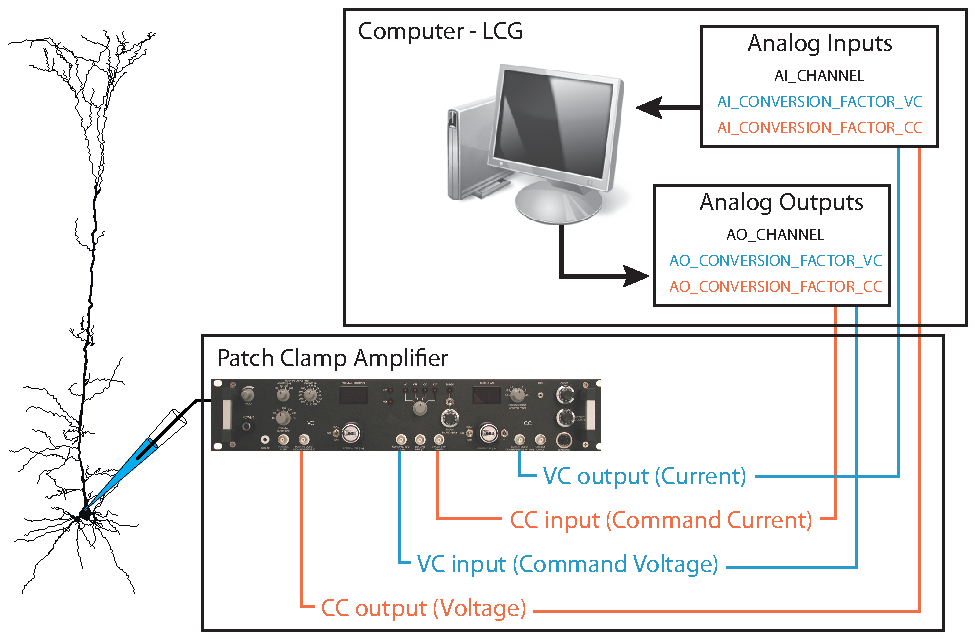
\includegraphics[width=0.8\textwidth]{figures/daq2amplifier}
    \caption{Correspondence between digital data acquisition board and the patch clamp amplifier.}
    \label{fig:daq2amplifier}
\end{figure}

Figure \ref{fig:daq2amplifier} illustrates the most important connections and environment variables required to control the amplifier both in current clamp and in voltage clamp mode. Protocols run in current clamp mode use the environment variables with \textbf{CC} suffix while those run in voltage clamp mode use the \textbf{VC} suffix. This allows different gains, channels and units to be used with minimal interaction from the user side.
 
The majority of \progname commands make sense in current clamp mode and therefore use the corresponding conversion factors. However, those  protocols that can be used both in voltage and current clamp modes (for instance, the steps protocol described before) use by default the current clamp conversion factors, but have an additional \texttt{--voltage-clamp} switch that instructs the command to use the corresponding conversion factors.
%
A command called \texttt{lcg-find-conversion-factors} can help
discovering the conversion factors associated with the patch clamp
amplifier.

It is important to remember that \progname cannot change the
conversion factors of the amplifier, which, from \progname point of
view, is simply a black box that sends and receives electrical
signals. Therefore, any changes in the conversion factors \textbf{on
  the amplifier} need to be matched by equivalent changes in the text
file that exports the environment variables used by \progname. If you
followed the installation instructions detailed in
Chap.~\ref{chap:installation}, this file is called
\texttt{.lcg-env.sh} and can be found in the home directory of the
user that performs the experiments.

\section{Your first recording}
Once you have configured the environmental variables as described in
section \ref{sec:configuration}, \progname is ready to be used for
patch clamp recordings. We can now attempt to characterize the V-I and
f-I curves of a real cell as we did for the LIF neuron at the
beginning of this chapter. This can be accomplished simply by running
the \texttt{lcg-steps} protocol. \newline
Set the amplifier to current clamp (CC) mode and enable the external
command (if required by the patch clamp amplifier). You can now use
the Active Electrode Compensation to compensate pipette resistance
errors so do not apply bridge compensation in the
amplifier\footnote{If you do not wish to use Active Electrode
  Compensation use the \texttt{--no-kernel} switch.}.

Go to the proper recording folder (\texttt{<folder name>/steps/01} in
the previous example) and type the following command:
 \begin{lstlisting}[language=bash]
lcg-steps -a -200,500,50  -d 1 
# Plot the results
lcg-plot -f all -k kernel.dat
\end{lstlisting}
%
This will first inject noise into the cell to compute the kernel that will be used for the offline Active Electrode Compensation and prompt the user for the number of points that are to be considered the length of the Electrode Kernel. 
Type a number so that the kernel encompasses the large peak and its decay. If you intend to use Active Electrode Compensation you should read \cite{Brette:2008}.
%
After extracting the electrode kernel the protocol will deliver shuffled current pulses between $-200$ and $500\,\pico\ampere$ in $50\,\pico\ampere$ steps.
%
All traces can be plotted using the \texttt{lcg-plot -f all} command with the \texttt{-k kernel.dat} option that indicates the kernel file to use.
%
\progname also provides functions (for \matlab and Python) to perform the Active Electrode Compensation offline.

%%%%%%%%%%%%%%%%%% COMMENT TRASH TEXT %%%%%%%%%
%\iffalse
%
%The example \ref{gettingStarted:example0} can solely help you check that \texttt{\progname} is installed, but it does not record/log anything on the disk. One way to save data is to use a Recorder object such as the \nameref{entity:H5Recorder}.
%
%
%
%
%
%Lets then extend the previous example by adding a \nameref{entity:H5Recorder} entity to the \texttt{entities} layer. 
%
%%The example \ref{gettingStarted:example0} can solely help you check
%%that \texttt{\progname} is installed, but it does not record/log
%%anything on the disk. One way to save data is to use a Recorder object
%%such as the \nameref{entity:H5Recorder}.
%%
%%Lets then extend the previous example by adding a
%%\nameref{entity:H5Recorder} entity to the \texttt{entities} layer.
%
%Note that the global \texttt{id} of the \texttt{H5Recorder} is
%different from the \texttt{LIFNeuron}, it is mandatory that all
%entities have a different global \texttt{id}.
%
%\begin{lstlisting}[caption={Example of a configuration file with a the H5Recorder entity.},label={gettingStarted:example1},language=XML,morekeywords={dynamic clamp,entities,entity,name,id,filename,compress,C,tau,tarp,Er,E0,Vth,Iext,parameters,connections,simulation,tend,rate}]]
%<dynamicclamp>
%  <entities>
%  	<entity>
% 	       <name>H5Recorder</name>
%        	<id>0</id>
%        	<parameters>
%		      <filename>example1.h5</filename>
%		      <compress>true</compress>
%	       </parameters>
%    	</entity>
%    	<entity>
%      		<name>LIFNeuron</name>
%      		<id>1</id>
%      		<parameters>
%			<C>0.08</C>
%			<tau>0.0075</tau>
%			<tarp>0.0014</tarp>
%			<Er>-65.2</Er>
%			<E0>-70</E0>
%			<Vth>-50</Vth>
%			<Iext>220</Iext>
%      		</parameters>
%      		<connections>0</connections>
%    	</entity>
%  </entities>
%  <simulation>
%  	<tend>5</tend>
%   	<rate>20000</rate>
%  </simulation>
%</dynamicclamp>
%
%\end{lstlisting}
%
%As for the example \ref{gettingStarted:example0}, create a file called
%\texttt{example1.xml}  - \inlineCode{gedit example1.xml};and copy the
%example \ref{gettingStarted:example1} to this file. Check which files
%are in this directory; you can do this with the command \texttt{ls} -
%check the \nameref{appendix:unixReference} for help on UNIX
%commands. To run the file use:
%\begin{lstlisting}[escapeinside=\{\}]
%{\progname} -c example1.xml
%\end{lstlisting}
%
%This will now create a file named \texttt{example1.h5} (use \texttt{ls}) to check for this.
%
%One of the most important advantages with using a
%realtime kernel is that the data analysis can be done on the same
%machine (as opposed to the target - host architectures that are
%typical of high performance realtime systems), and since it uses
%priorities you can even do the analysis (virtually) at the same time
%you are running a realtime task. We will now see how to use
%\textbf{\matlab} to read this file and extract the timing of the
%spikes. 
%
%First open \matlab in a terminal window with the command: 
%\begin{lstlisting} 
%matlab -nodesktop 
%\end{lstlisting}
%
%You should see something like:
%\begin{lstlisting}[numbers=none,language=xml]
%		< M A T L A B (R) >
%Copyright 1984-2012 The MathWorks, Inc.
%	R2012b (8.0.0.783) 64-bit (maci64)
%		August 22, 2012
%
%To get started, type one of these: helpwin, helpdesk, or demo.
%For product information, visit www.mathworks.com.
% 
%>> 
%\end{lstlisting}
%
%We will use \matlab without desktop in these examples if you prefer
%to use the desktop mode, you can launch \matlab with the command
%\inlineCode{matlab &}; all this assuming \matlab binaries have been
%added to path.
%
%%\paragraph{}
%\matlab can be used to automate the analysis method in a highly
%efficient manner however in this section we will focus on the basic
%concepts. Rest assured: once you get a grip of \matlab and \matlab
%functions you will greatly reduce the amount of time that you require
%to analyse these sort of traces.
%
%\subsection{\matlab functions and the path}
%%\paragraph{}
%You could load these file only using the built in functions of
%\matlab to read HDF5 files however this would be rather time
%consuming. The basic notions of \matlab that you need to get
%acquainted with before continuing the are the concept of
%\texttt{functions} and \texttt{path}.
%%\paragraph{}
%The terminal that you have in front of you is interactive and the
%commands you type there will be ran as \matlab commands. Some of the
%power of \matlab lays in how simple it is to create functions. A
%function can be seen as a generic box that receives inputs and returns
%outputs. The computations processed to transform the inputs into the
%outputs are the core of the function. In \matlab functions are defined
%by naming a file with the name of the function and placing the code
%\inlineCode{function [out] = functionName(in)} in the first line of
%that file.
%
%%\paragraph{}
%This said, \matlab functions are just files which are named as the
%function. \matlab does not search for functions in all directories of
%your disk (this is a good thing!) and because of that you have to tell
%\matlab where to search for functions. In order to do so you can use
%the \texttt{add path} command.
%
%Every \matlab function/command has a documentation built in. You can
%access this by typing \inlineCode{help <name>}.
%
%Now you need to add the functions that ship with \progname\ to the
%path (in case they are not already there). You can do this (for the
%current \matlab session) by doing:
%
%\begin{lstlisting}[escapeinside=\{\}]
%addpath([getenv('{\progname}_path'),'\matlab'])
%\end{lstlisting}
%
%Note that the above command will not work if you haven't defined the
%variable \texttt{\progname\_path} in your environment
%(\texttt{\$HOME/.bashrc} file) as the location of the source code of
%\progname. Although this command may seem complicated to the first
%time user of \matlab, the only thing it does is retrieving the
%environment variable '\texttt{\progname\_path}' and concatenating it
%with the \texttt{'\textbackslash matlab'} string. This because the we
%want to add the files that are in this folder to the \matlab path.
%
%\subsection{Loading and plotting the recorded traces}
%
%Now that you added the function in the source path of \progname\ to
%the path of \matlab with the command:
%
%\begin{lstlisting}[escapeinside=\{\}]
%addpath([getenv('{\progname}_path'),'\matlab'])
%\end{lstlisting}
%
%The function \texttt{loadH5Trace} will be available for \matlab. Type
%\inlineCode{help loadH5Trace} to access the help of this function.
%You can load and plot the data with the commands:
%
%\begin{lstlisting}[language=matlab,morekeywords={loadH5Trace,ls},escapeinside=\{\}]
%files = dir({\textquotesingle}*.h5{\textquotesingle});
%[entities,info] = loadH5Trace(files(1).name)
%entities(1).name
%Vm = entities(1).data;
%time = [0:length(Vm)-1]*info.dt;
%plot(time,Vm,{\textquotesingle}k{\textquotesingle})
%\end{lstlisting}
%
%The first line uses \matlab's command \texttt{dir} to list all
%directories. Then \texttt{loadH5Trace} loads the data into the
%variables \texttt{entities} and \texttt{info} -  it loads one
%structure per entity connected to the \nameref{entity:H5Recorder}
%and thus we will think of it as a structure array (read about \matlab
%datatypes).
%
%The third line in the above code is solely for illustration of how you
%can find out the name of an entity in the \texttt{entities}
%array. This can be particularly useful since it lets you find a
%particular entity based on it's type. Later we will see how to take
%advantage of this feature.
%The fourth and fifth line we associate the variable Vm to the recorded
%membrane potential of the \nameref{entity:LIFNeuron} and create a
%time vector with the size of \texttt{Vm} and using the time step that
%is saved in the \texttt{info} structure.
%
%The last line plots the time versus the voltage using the colour black.
%
%\subsection{Detecting the peak of the spikes}
%
%There are several ways of detecting the peaks of the spikes. We will
%focus on a relatively robust yet simple method of doing so by taking
%advantage of the \matlab function \texttt{findpeaks}.
%
%\begin{lstlisting}[language=matlab,morekeywords={findpeaks,THRESHOLD,MINPEAKDISTANCE},escapeinside=\{\}]
%% Define the refractory period of the peak detector (1ms); this can be useful when dealing with noisy signals.
%refractory = 1.e-3/info.dt; 
%% The following uses the function find peaks to find the spikes with threshold crossing at 0mV and a refractory period. 
%[peaks, loc] = findpeaks(Vm,{\textquotesingle}THRESHOLD{\textquotesingle},0,{\textquotesingle}MINPEAKDISTANCE{\textquotesingle},refractory);
%% The spikes are the locations of the peaks on the time vector
%spks = time(loc);
%% Plot time versus membrane potential
%plot(time, Vm,{\textquotesingle}k{\textquotesingle})
%hold on
%% Plot the spike times and the peaks of the Action Potentials. The {\textquotesingle}hold on{\textquotesingle} command makes that the plots overlap.
%plot(spks, peaks,{\textquotesingle}b.{\textquotesingle})
%\end{lstlisting}
%
%The above commands will get you to extract the peaks of the action
%potentials and the spike times and to plot them on the membrane
%voltage trace.
%These commands should work also with very noisy signals, as long as
%the threshold and the refractory period are defined accordingly.
%
%%\paragraph{}
%Now it would be useful to know the mean interspike interval. First we
%need to compute the interspike intervals, that can be easily done by
%using the \texttt{diff} command. 
%
%\begin{lstlisting}[language=matlab,morekeywords={findpeaks,THRESHOLD,MINPEAKDISTANCE},escapeinside=\{\}]
%% Compute te interspike intervals
%isi = diff(spks);
%% And the mean can be computed in a straight forward manner:
%mean(isi)
%% The reciprocal will give you the result in Hz
%1./mean(isi)
%\end{lstlisting}
%
%\section{Adding stimulation}
%%\paragraph{}
%Intracellular or virtually every form of stimulation or pulse
%triggering can be done with \progname. In this section we will
%introduce the \nameref{entity:Waveform} entity.
%The \nameref{entity:Waveform} entity interfaces with Stimulus
%Generator Library - see appendix \ref{appendix:stimgen}; in short an
%elementary waveform (and linear combinations of elementary waveforms)
%can be represented by 12 numbers:
%
%\begin{center}
%\footnotesize\ttfamily
%\begin{tabular}{rrrrrrrrrrrr}
%[T & CODE & P1 & P2 & P3 & P & P1 & FIXSEED & MYSEED & SUBCODE & OPERATOR & EXPON]
%\end{tabular}
%\end{center}
%
%The waveform types range from constant values to double exponential
%decays and stochastic processes realisations. In order to start using
%the \nameref{entity:Waveform} entity lets consider the example
%\ref{gettingStarted:example1} and add one more entity as bellow:
%
%\begin{lstlisting}[caption={Example of a configuration file with a the \nameref{entity:Waveform} entity.},label={gettingStarted:example2}, language=XML,morekeywords={dynamic clamp,entities,entity,name,id,filename,compress,C,tau,tarp,Er,E0,Vth,Iext,parameters,connections,simulation,tend,rate}]
%<dynamicclamp>
%  <entities>
%  	<entity>
% 	       <name>H5Recorder</name>
%        	<id>0</id>
%        	<parameters>
%		      <filename>example2.h5</filename>
%		      <compress>true</compress>
%	       </parameters>
%    	</entity>
%    	<entity>
%      		<name>LIFNeuron</name>
%      		<id>1</id>
%      		<parameters>
%			<C>0.08</C>
%			<tau>0.0075</tau>
%			<tarp>0.0014</tarp>
%			<Er>-65.2</Er>
%			<E0>-70</E0>
%			<Vth>-50</Vth>
%			<Iext>220</Iext>
%      		</parameters>
%      		<connections>0</connections>
%    	</entity>
%    	<entity>
%      		<name>Waveform</name>
%      		<id>2</id>
%      		<parameters>
%			<filename>current.stim</filename>
%      		</parameters>
%      		<connections>0,1</connections>
%    	</entity>	
%  </entities>
%  <simulation>
%  	<tend>5</tend>
%   	<rate>20000</rate>
%  </simulation>
%</dynamicclamp>
%
%\end{lstlisting}
%
%%\paragraph{}
%We connected the \nameref{entity:Waveform} entity (2) to both the
%\nameref{entity:LIFNeuron} (1) and the \nameref{entity:H5Recorder}
%(0). In this way we can both stimulate the neuron (current injection)
%and record the stimulation trace; as well as the response of the
%neuron as it is connected to the \nameref{entity:H5Recorder} (0).
%You can see that the Waveform has a parameter \texttt{filename} that
%points to  "current.stim" where the stimulus is described using the
%\nameref{appendix:stimgen} nomenclature.
%
%%\paragraph{}
%Now lets create a file named \texttt{current.stim} using \texttt{gedit
%  current.stim}. Copy and paste the following lines to it:
%\begin{center}
%\ttfamily
%\begin{tabular}{rrrrrrrrrrrr}
%2 & 1 & 0.0 & 0 & 0 & 0 & 0 & 0 & 0 & 0 &0 & 1 \\
%1 & 1 & 200.0 & 0 & 0 & 0 & 0 & 0 & 0 & 0 & 0 & 1 \\
%2 & 1 & 0.0 & 0 & 0 & 0 & 0 & 0 & 0 & 0 & 0 & 1 \\
%\end{tabular}
%\end{center}
%
%%\paragraph{}
%Note the second row (that represents the code of the elementary
%waveform) uses \textbf{code 1} in all lines: this stands for a DC or
%stationary current.
%The first line has a duration of 2 seconds (first row) with amplitude
%(third row) 0; is followed by 1 second of amplitude 200 (pA)
%\footnote{The convention of the \nameref{entity:LIFNeuron} is that
%  it's inputs units are the pico ampere (pA).} and by again 2 seconds
%of amplitude zero. Since the stimulation lasts 5 seconds this will
%just cause a pulse of 200pA and 1 second duration after a baseline
%recording for 2 seconds. 
% 
%%\paragraph{}
%Lets now copy example \ref{gettingStarted:example2} to a file
%(\texttt{gedit example2.xml}) and run this simulation
%(\texttt{\progname\ -c example2.xml}).
%
%The result has been saved into the \texttt{example2.h5} file. We will
%now analyse this data with \matlab.
% 
%%\paragraph{}
%As for the previous section open \matlab (\texttt{matlab -nodesktop})
%and using the interactive mode lets plot the results and detect the
%spikes\footnote{Remember that in \matlab text that follows the percent
%  sign (\%) are just comments and will hence be ignored.}.
% 
%\begin{lstlisting}[language=matlab,morekeywords={loadH5Trace,ls},escapeinside=\{\}]
%% List files that follow the filter *.h5
%files = dir({\textquotesingle}*.h5{\textquotesingle})
%% Load the second trace (example2.h5) file
%[entities,info] = loadH5Trace(files(2).name)
%% Display the name of the entities
%{\{} entities.name {\}}
%% The voltage is in entity 1 given the order that the entities were specified.
%Vm = entities(1).data;
%% And the current (I) will be from the waveform.
%I = entities(2).data;
%% Generate a time vector
%time = [0:length(Vm)-1]*info.dt;
%% Make 2 plots in a figure 
%subplot(2,1,1)
%% One for the membrane voltage
%plot(time,Vm,{\textquotesingle}k{\textquotesingle})
%% And another for the injected current
%subplot(2,1,2)
%plot(time,I,{\textquotesingle}r{\textquotesingle})
%% Detect the time of the spike peaks.
%refractory = 1.e-3/info.dt; 
%% The following uses the function find peaks to find the spikes with threshold crossing at 0mV and a refractory period. 
%[peaks, loc] = findpeaks(Vm,{\textquotesingle}THRESHOLD{\textquotesingle},0,{\textquotesingle}MINPEAKDISTANCE{\textquotesingle},refractory);
%% The spikes are the locations of the peaks on the time vector
%spks = time(loc);
%% Plot on the voltage plot (you need to use hold on to keep the previous plot)
%subplot(2,1,1)
%hold on
%% Plot the spike times and the peaks of the Action Potentials. The {\textquotesingle}hold on{\textquotesingle} command makes that the plots overlap.
%plot(spks, peaks,{\textquotesingle}b.{\textquotesingle})
%\end{lstlisting}
% \fi
%% END OF COMMENT OUT
%%%%%%%%%%%%%%%%%%%%%%%%%%%%%%%%%%%%%%%%%%%
 
